\documentclass[12pt]{article}
\usepackage{graphicx}
\usepackage{epstopdf}
\usepackage{listings}
\usepackage[backend=bibtex,style=alphabetic,natbib=true]{biblatex} % (which resembles APA)
\usepackage{hyperref}
\hypersetup{
    colorlinks=true,
    linkcolor=blue,
    filecolor=magenta,      
    urlcolor=cyan,
}
 
\urlstyle{same}
\addbibresource{kcorebip.bib} % The filename of the bibliography

\title{Using the kcorebip package \\ \small{Version 0.1}}
\author{Javier Garcia-Algarra \\ \href{mailto:jgalgarra@coit.es}{jgalgarra@coit.es} }

\begin{document}

\flushbottom
\maketitle
\thispagestyle{empty}

\section*{Introduction}

This package performs the \textit{k-core decomposition} analysis of a bipartite graph and provides two new kinds of plot: \textit{polar} and \textit{ziggurat}. It works for
any kind of bipartite network, but we developed it to study ecological mutualistic communities, so we use terminology and examples of that research field.

\section*{Decomposition and definition of k-magnitudes}
\label{K-magnitudes}

The \textit{k-decomposition} is an iterative algorithm that prunes links of nodes with degree equal or less than $k$ \cite{seidman1983network}. The process starts pruning nodes with $k=1$ until all the resting nodes have two or more links. Then it continues with $k=2$, and so on. After performing the \textit{k-decomposition}, each species belongs to one of the \textit{k-shells}. The highest value of \textit{k}, i.e $ks_{max}$, corresponds to the innermost \textit{core} $ks_{max}\equiv C^{A,B}$. For each \textit{k-shell} there are two subsets, one per guild ($A$ and $B$), that we call $K^{A}_{j}, K^{B}_{j}$ where $j$ is the \textit{k-shell} index.

In order to quantify the distance from a node to the innermost shell of the partner guild, we calculate the average of the shortest paths to all the nodes in that set. We define the \textit{$k_{radius}$} of node $m$ of class $A$ as the average distance to the species of $C^B$:

\begin{equation}
\displaystyle
k^A_{radius}(m) = \frac{1}{\mid C^{B} \mid}\sum\limits_{j \in C^{B}} dist_{mj}  \qquad   m \in A
\label{kradius}
\end{equation}

\noindent where $dist_{mj}$ is the shortest path from species $m$ to each of the $j$ species that belong to the set $C^B$. The same definition is valid for species of the guild $B$ computing the average distance to $C^A$. The minimum possible radius value is $1$ for one node of the maximum shell directly linked to each one of the maximum shell set of the opposite guild.

\begin{figure}[h!]
\centering
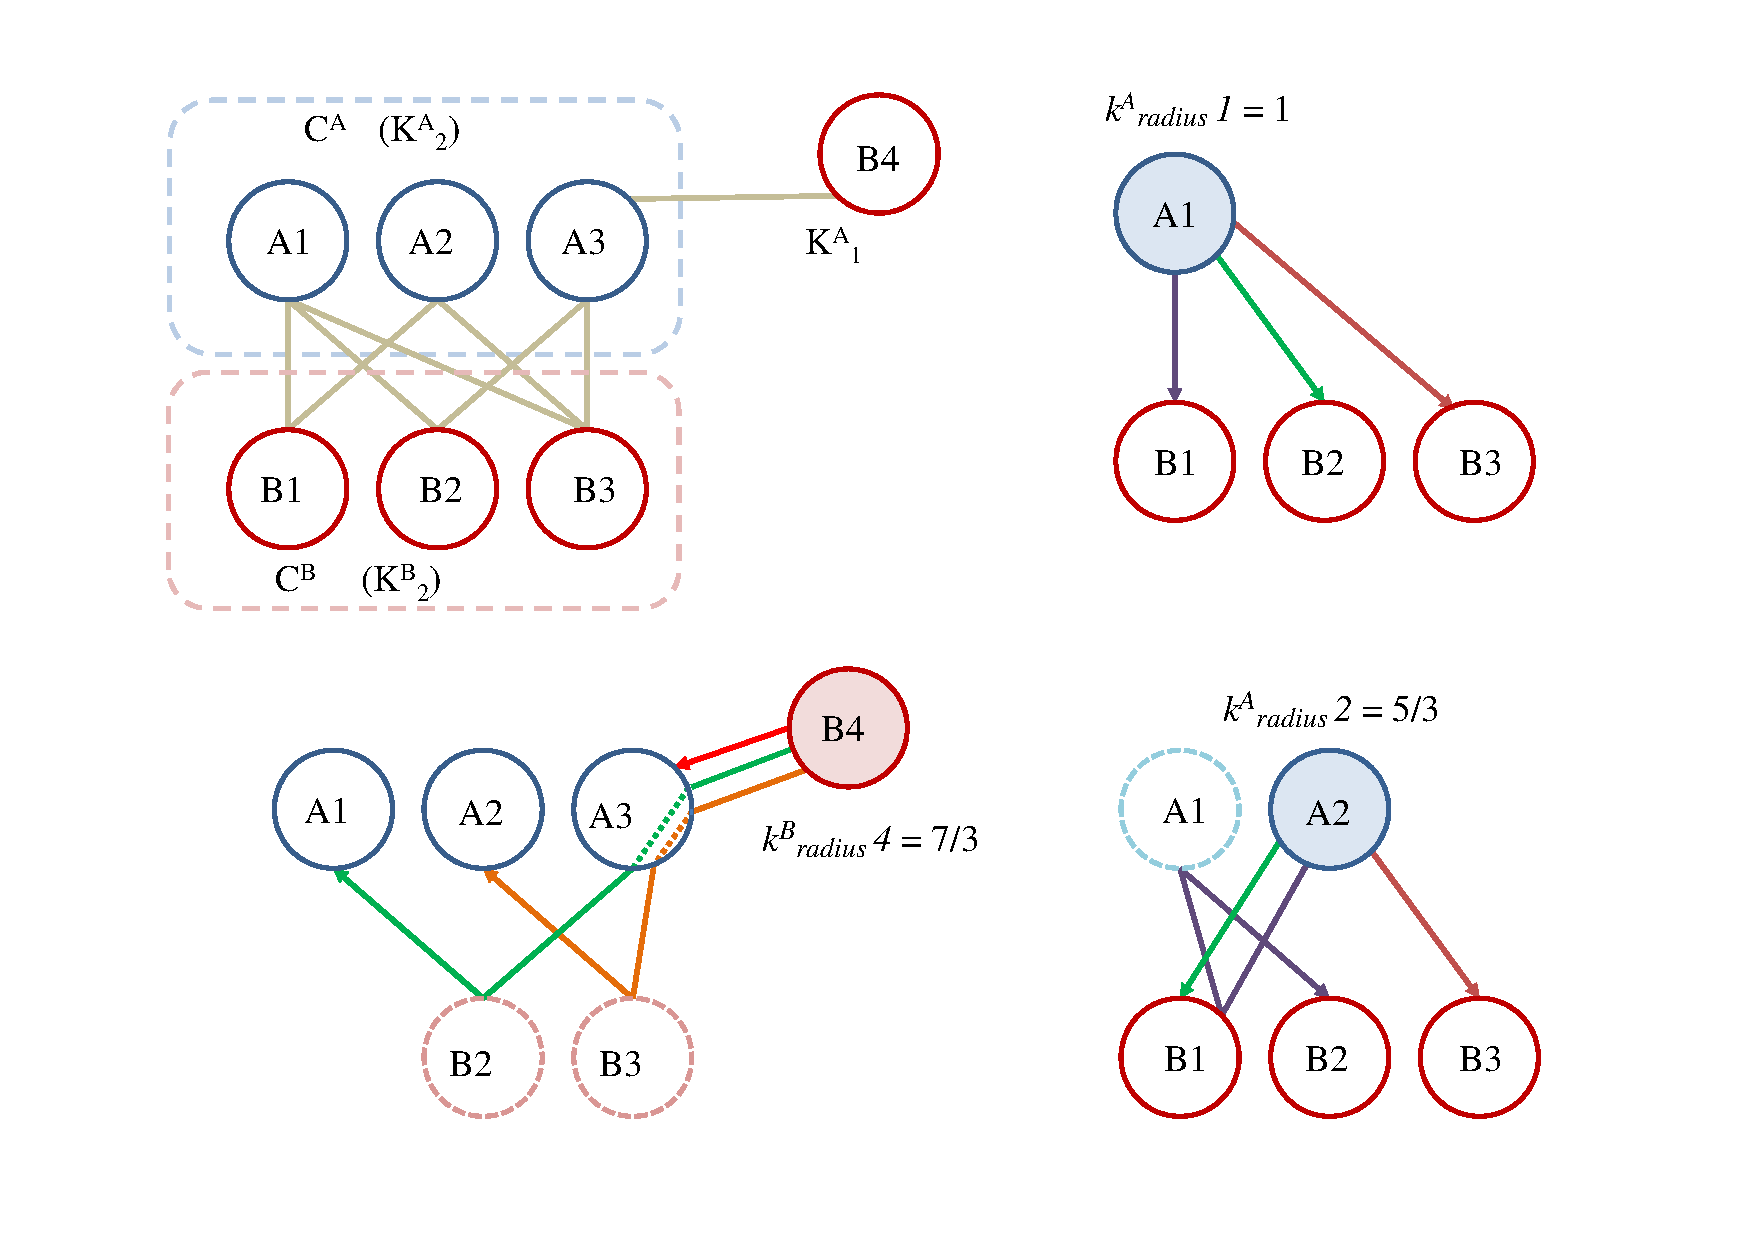
\includegraphics[scale=0.4]{red_example.pdf}
\caption {Examples of \textit{$k_{radius}$} in a fictional network.}
\label{fig:red_example}
\end{figure}

Figure \ref{fig:red_example} is a very simple fictional network, with only seven nodes. The upper left graph shows network structure. In the upper right figure, species $A1$ belongs to $C^{A}$.  The distance to each of the nodes of $C^{B}$ is $1$, so its \textit{$k_{radius1}(1)$} is $1$. In the bottom right figure, node  $A2$ also belongs to $C^{A}$ but there is not any direct link with $B2$, so the distance between them is $3$ and \textit{$k_{radius}(2)$} is $\frac{5}{3}$. In the bottom left figure, node $B4$ is not part of $C^{B}$, and as may be expected, the value of its \textit{$k_{radius}$} is higher. 

A global value can be defined averaging this magnitude across network:

\begin{equation}
\displaystyle
\overline {k}_{radius} = \frac{1}{\mid A \cup B \mid}\sum\limits_{l \in A \cup B} k_{radius}(l)
\label{avgkradius}
\end{equation}

In our example network of Figure \ref{fig:red_example}, the value is $11/7$. 

${k}_{radius}$ is a useful magnitude to measure network compactness but it not a good measure of centrality. For instance, its value for an isolated specialist linked to the maximum core is low. \emph{To attend this necessity,} we define a second \textit{k-magnitude}, the ${k}_{degree}$:

\begin{equation}
\displaystyle
k^A_{degree}(m) = \sum\limits_{j} \frac{a_{mj} }{k_{radius}j}  \quad   m \in A, \forall j \in B
\label{kdegree}
\end{equation}

\noindent where $a_{mj}$ is the element of the interaction matrix that represents the link. So the $k_{degree}m$ is the sum of the inverse of $k_{radius}$ for each node linked to $m$. A node of the innermost shell will have a high degree, whereas specialists have only one or two links and so a low $k_{degree}$. In the example of Figure \ref{fig:red_example}, this magnitude is $1+3/5+3/5 = 11/5$ for node $B3$, while only $3/7$ for node $B4$. 

\subsection*{Input file format}
\label{input_file_format}

We use the file format of \href{http://www.web-of-life.es/}{web of life} ecological data collection \cite{bascompte2009}. Data are stored as \texttt{.csv} files. Species of guild \textit{a} are distributed by colums, and those of guild \textit{b} by rows. First colum contains the labels of guild b nodes, and first row, the labels of guild a. If the interaction matrix is binary, the cell of $species\_a\_m,species\_b\_n$ will be set to 1. If it is weighted, to a real number different of 0.

The naming convention is $M\_XX\_NNN.csv$ where $XX$ is the type, $PL$ for pollinator networks and $SD$ for seed dispersers, and $NNN$ a serial number. Anyway, you can call your file whatever you want.

\begin{figure}[h!]
\centering
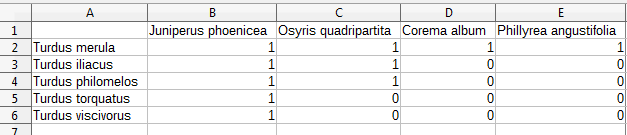
\includegraphics[scale=0.8]{SD_029_csv.png}
\caption {Examples of input file, the seed disperser network $029$ of \href{http://www.web-of-life.es/}{web of life} site.}
\label{fig:red_example}
\end{figure}

\subsection*{Network analysis}
\label{network_analysis}

The function \texttt{analyze\_network} performs the \textit{k-core decomposition} and analysis.


\fontsize{3.5mm}{3.5mm}\selectfont
\begin{verbatim}
analyze_network(namenetwork, directory = "", guild_a = "pl",
                guild_b = "pol", plot_graphs = FALSE, only_NODF = FALSE)
\end{verbatim}
\normalsize

Arguments:
\small
\begin{itemize}

\item \texttt{namenetwork}:  name of the file of the interaction matrix.
	
\item \texttt{directory}: where the network file is stored.

\item \texttt{guild\_a}: prefix for the guild of nodes stored in rows.

\item \texttt{guild\_b}: prefix for the guild of nodes stored in columns.

\item \texttt{plot\_graphs}: plot kshell histogram and Kamada Kawai plots.

\item \texttt{only\_NODF}: just computes the $NODF$ measurement of nestedness.

\end{itemize}

The function returns:
\begin{itemize}
\item \texttt{calc\_values}, a list containing the following objects:
   \begin{itemize}
   
\item \texttt{graph}: an igraph::graph object

\item \texttt{max\_xore}: maximum k shell index

\item \texttt{nested\_values}: a list containing all the values provided by the bipartite::nested function, unless \texttt{only\_NODF} set TRUE.

\item \texttt{num\_guild\_a}: number of nodes of guild a.

\item \texttt{num\_guild\_b}: number of nodes of guild b.

\item \texttt{links}: number of network links.

\item \texttt{meandist}: network average kradius.

\item \texttt{meankdegree}: network average kdegree.

\item \texttt{spaths\_mat}: matrix with node to node shortest distance paths.

\item \texttt{matrix}: adyacency matrix with nodes of guild a by columns and guild b by rows.

\item \texttt{g\_cores}: list with the value of kshell for each node.

\item \texttt{modularity\_measure}: value of igraph::modularity function.
   \end{itemize}


\end{itemize}

\clearpage
\subsection*{The Polar Plot}
\label{polar_plot}

The \textit{Polar Plot} shows nodes (species) centrality and provides an overview of network distribution. It was inspired by the \textit{fingerprint-like} graph, developed by Alvarez-Hamelin \textit{et al.} \cite{alvarez2005k} to plot very large \textit{k-decomposed} networks.

Nodes are depicted with their centers located at $k_{radius}$. Angles are assigned at random by the visualization algorithm and each guild lies inside one of the half planes. The size of each node is proportional to its $k_{degree}$ and the color represents the $k_{shell}$. This visualization does not include links. The user may choose adding the histograms of \textit{k-magnitudes}, a handy option because they convey a wealth of structural information.

%Figure \ref{fig:red_example} is a real mid size network. A reduced number of nodes have a high $k_{degree}$, while most species are peripheral. 

\noindent The function call is:

\fontsize{3.5mm}{3.5mm}\selectfont
\begin{verbatim}
polar_graph <- function( red, directorystr = "data/", 
                         plotsdir = "plot_results/polar/", 
                         print_to_file = FALSE, pshowtext = FALSE,
                         show_histograms = TRUE, 
                         glabels = c("Plant", "Pollinator"),
                         gshortened = c("pl","pol"),
                         lsize_title = 22, lsize_axis = 12, 
                         lsize_legend = 13, lsize_axis_title = 14, 
                         lsize_legend_title = 15, file_name_append = "",
                         print_title = TRUE,
                         progress = NULL, printable_labels = 0)
\end{verbatim}
\normalsize

The parameters \texttt{red}, \texttt{directorystr} and \texttt{plotsdir} are the name of the adyacency matrix, the directory where it is stored and the name of the plotting directory. If \texttt{print\_to\_file} is set to \texttt{FALSE} the polar plot will be displayed in the current R session. The name of the output file is that of the input file
plus \texttt{\_polar.png}. Paths are relative to the current working path in \texttt{R} but you may also specify absolute paths.

File plots have a resolution of 600 dots per inch, and a size of 12 x 12 inches. If the user wants to display the result in the current R session, label sizes may appear different depending on the installed fonts and size of the plotting window.

The following command creates the file \texttt{M\_PL\_001\_polar.png} in the directory \texttt{graphresults/}

\fontsize{3.5mm}{3.5mm}\selectfont
\begin{verbatim}
polar_graph("M_PL_034.csv","data/",plotsdir="grafresults/",
            print_to_file = TRUE)
\end{verbatim}
\normalsize

\begin{figure}[h!]
\centering
\includegraphics[scale=0.4]{M_PL_034_polar.png}
%\caption {Examples of \textit{$k_{radius}$} in a fictional network.}
\label{fig:red_example}
\end{figure}

The plot title includes the network average ${k}_{radius}$ and ${k}_{degree}$, a common measurement of \textit{nestedness} called $NODF$ \cite{almeida2008consistent} and $Modularity$ following the \textit{QanBiMo} method \cite{dormann2014method}.

By default, nodes are unlabeled. You may choose to print some of them with the parameter \texttt{printable\_labels}, but have in mind that the
diagram may become messy. Guild labels are also configurable. The function will set automatically "Plant, Pollinator" and "Plant, Disperser" if the
file follows the naming convention of the web of life site; you may choose any other pair of values with the input parameter \texttt{glabels}.

Three histrogams are displayed under the main plot, with the distributions of $k_{radius}$, $k_{degree}$ and $k_{shell}$. 

The configuration of a polar graph is quite simple. The following picture shows how and where the different input parameters modify the plot.

\clearpage
\begin{figure}[ht!]
\centering
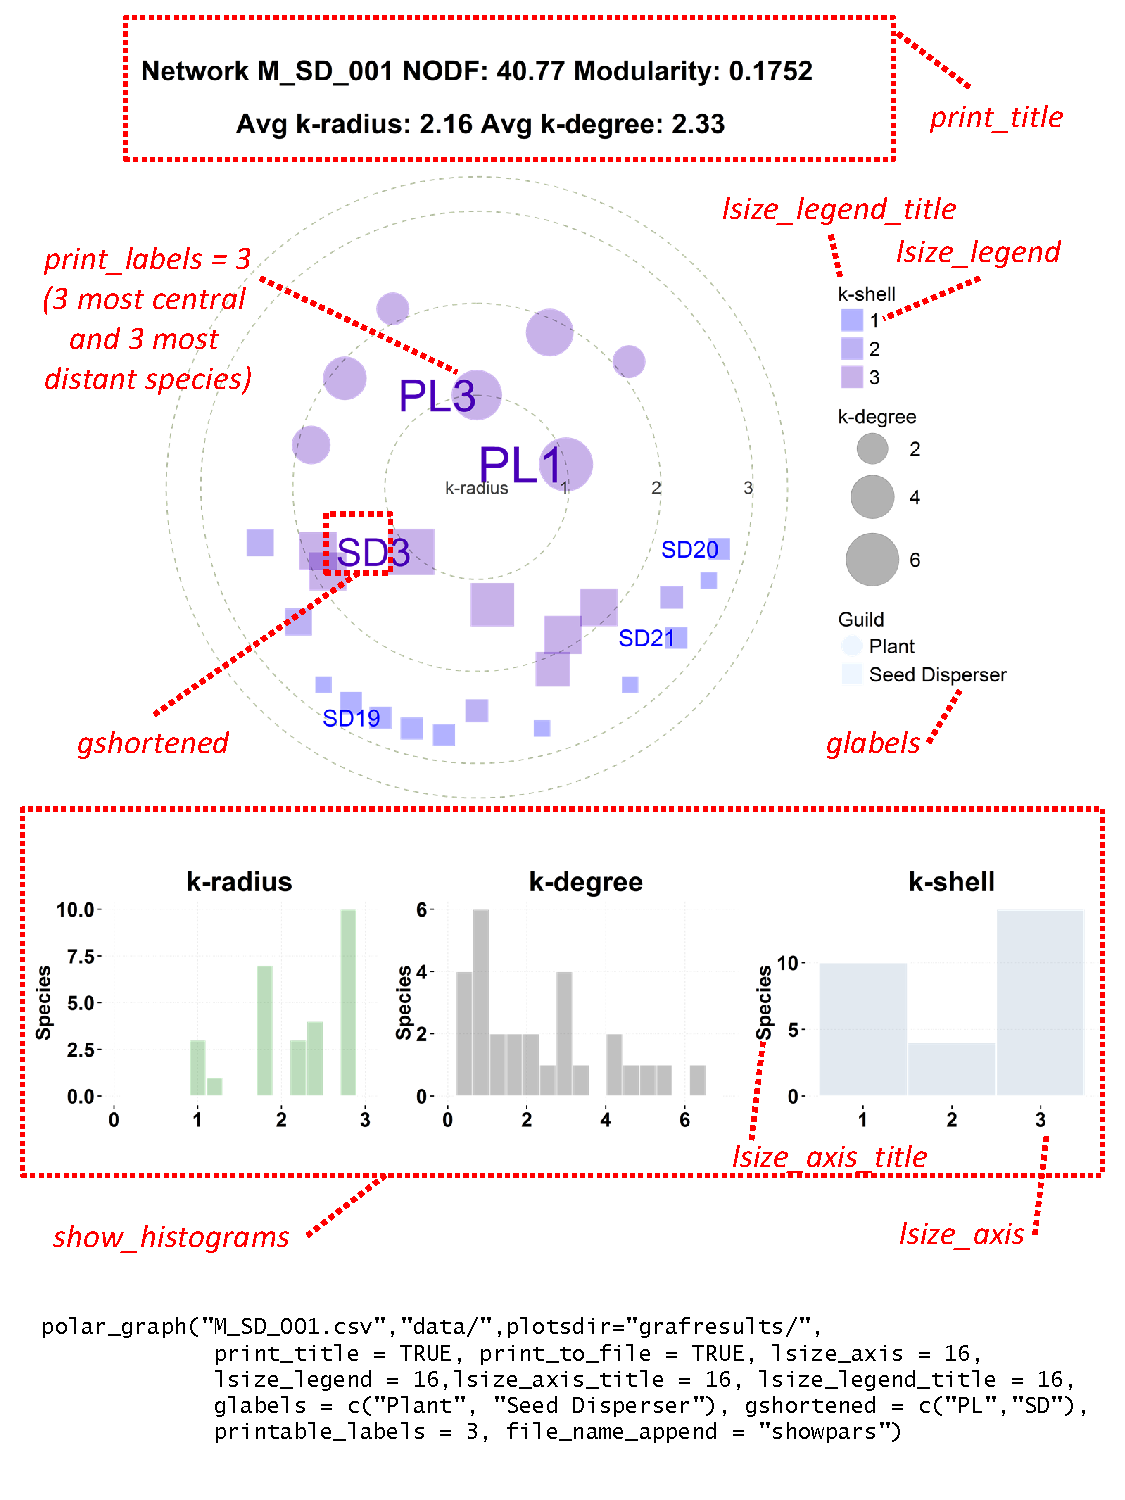
\includegraphics[scale=0.75]{polar_params.pdf}
\label{fig:polar_params}
\end{figure}

\clearpage

\subsection*{The Ziggurat Plot}
\label{polar_plot}

\textit{Ziggurat} is the second type of visualization, created from scratch. Species are grouped by their $k$-$shells$. Each of these groups are represented as small ziggurats. The maximum $k$-$shell$ is located on the left side, the other ones are arranged following an almond-like distribution. 

Species of the maximum shell are ordered by their $k_{degree}$ with the highest one leftmost. Areas do not convey meaning, their height decreases just by convenience of visualization. 

\begin{figure}[hp!]
\centering
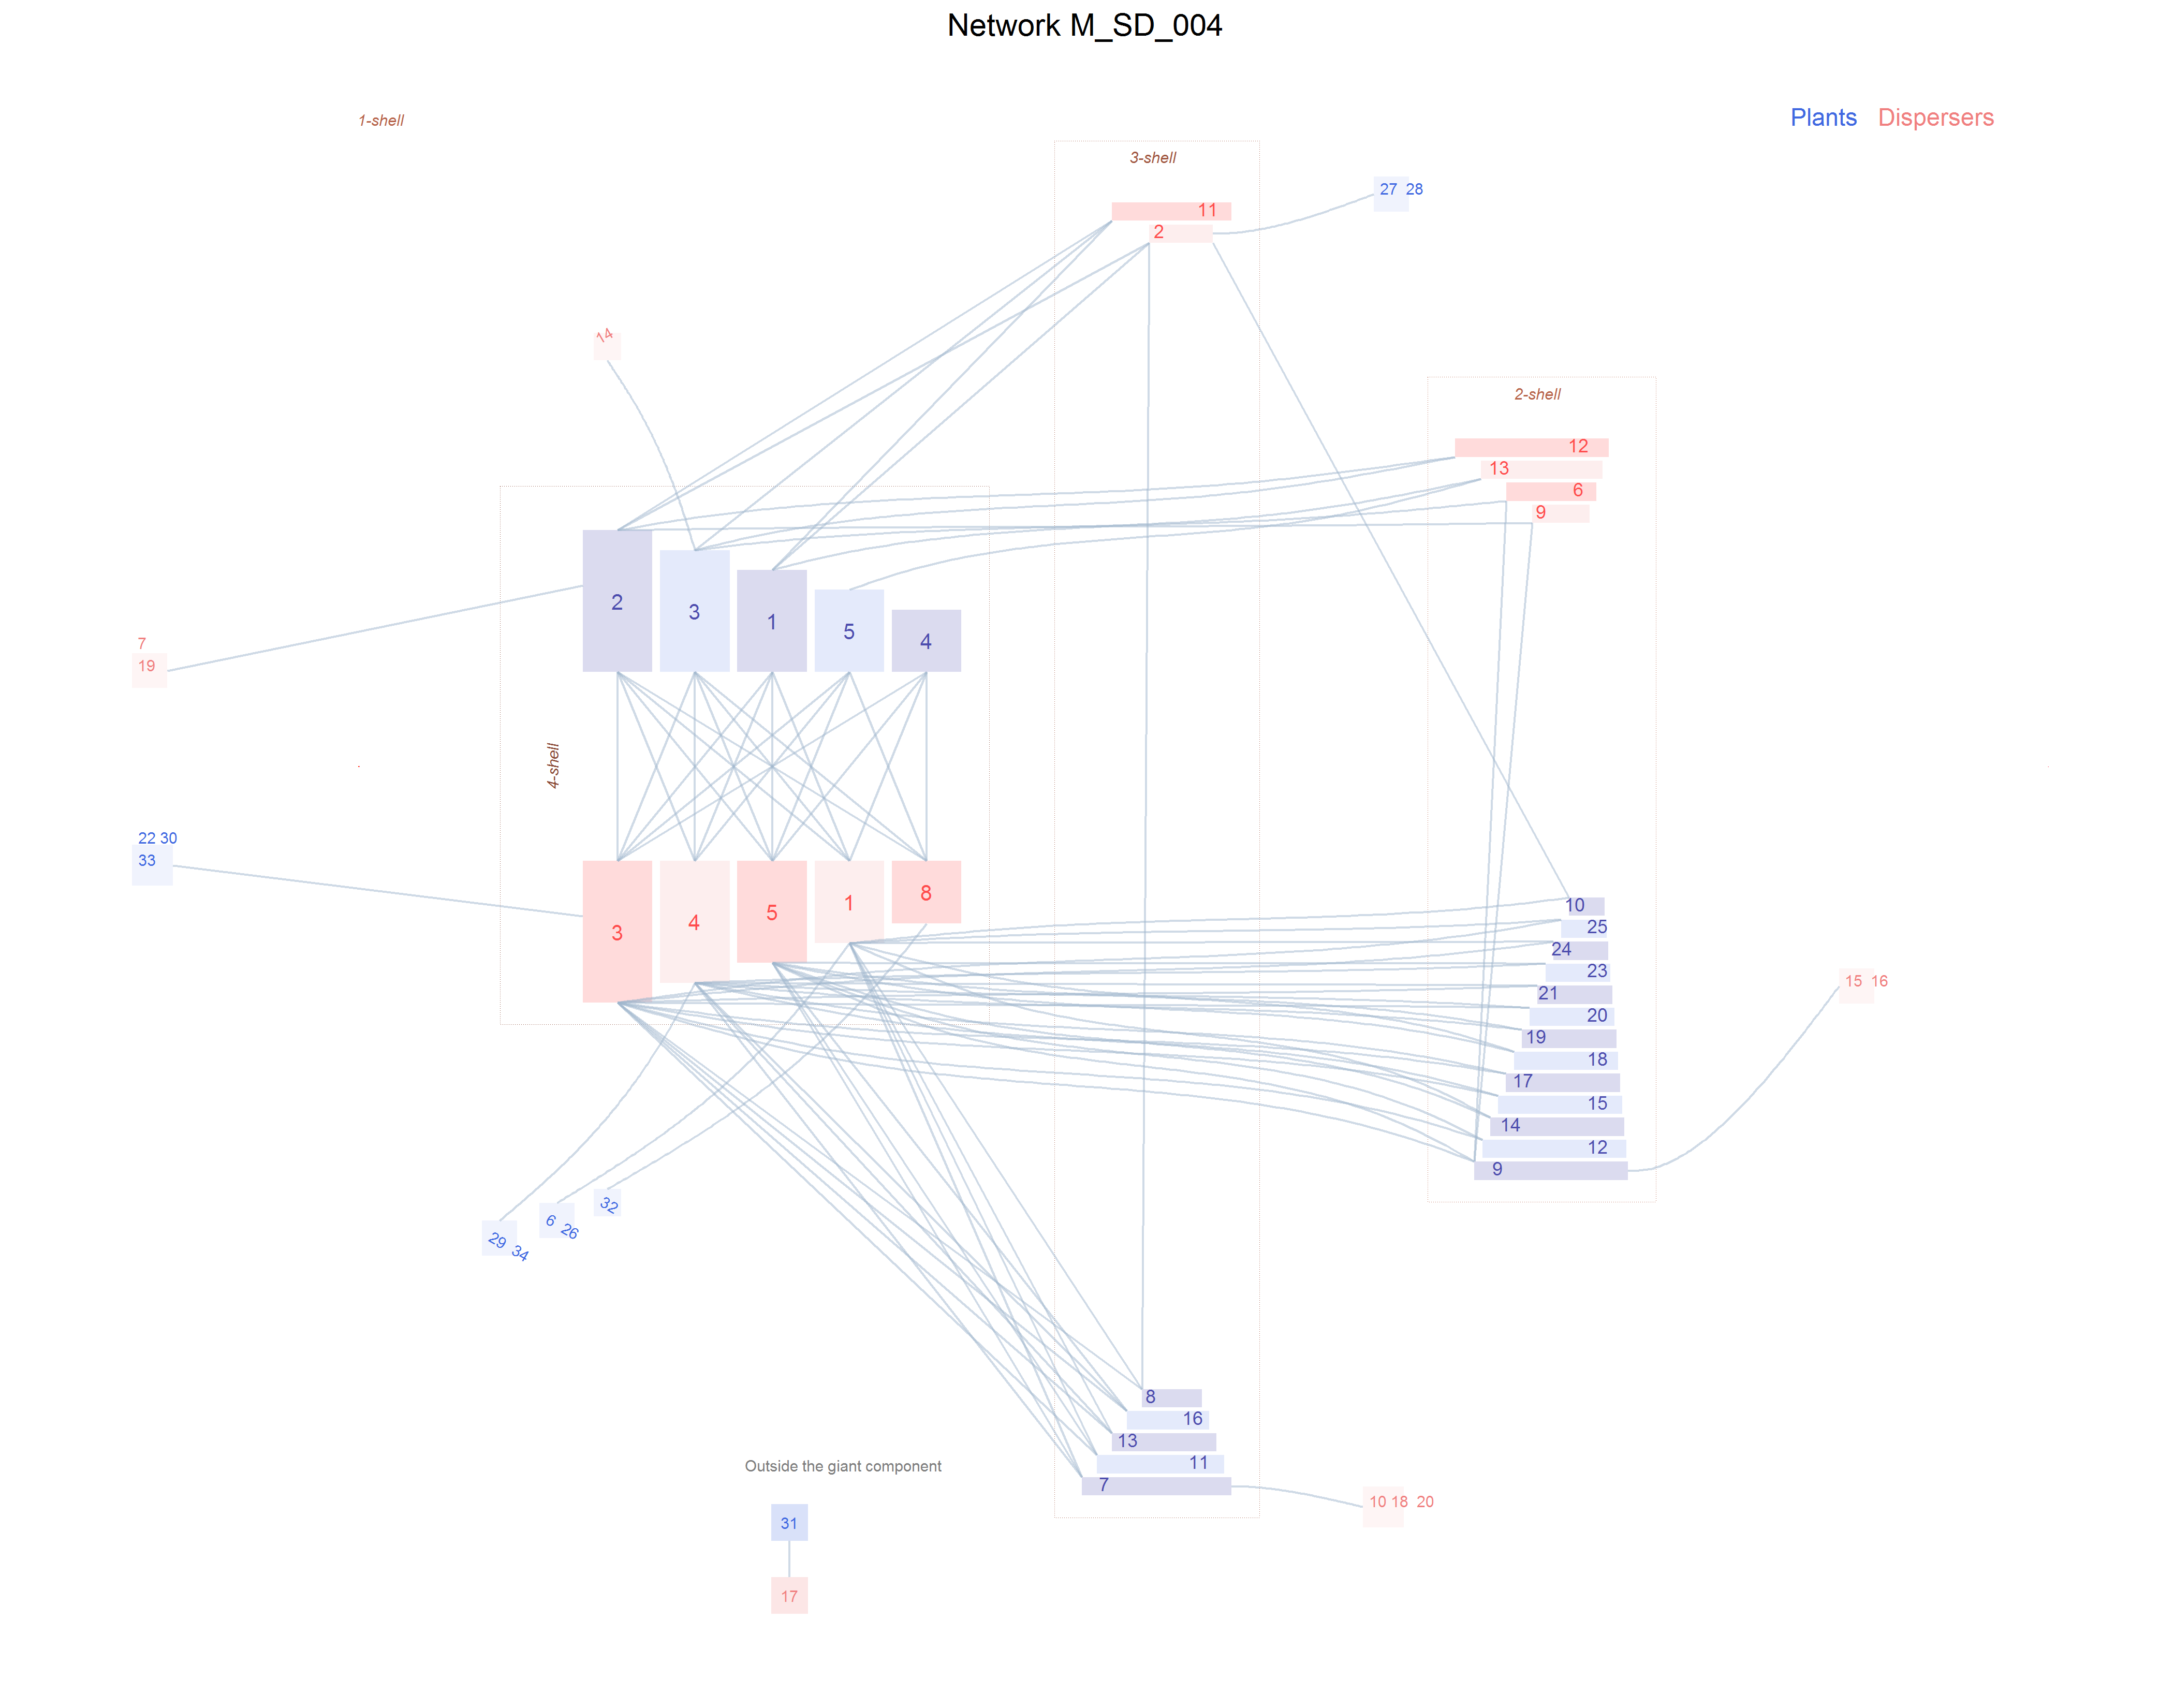
\includegraphics[scale=0.4]{M_SD_004_ziggurat.png}
\caption {Ziggurat graph of an avian frugivore community in Puerto Rico with 54 species and 95 links \cite{carlo2003avian}.}
\label{fig:ziggurat}
\end{figure}

Nodes of $1$-$shell$ are scattered around the ziggurats. When multiple species of this shell are connected to the same node of any of the ziggurats they are clustered to reduce the number of lines. For instance, plants species $22, 30$ and $33$ are specialists linked to the generalist disperser $3$. With this organization, we get a clear view of structure and interconnections. The almond shape leaves a wide space in the center of the graph to depict the links and they do not overcross the boxes of the different species.

\noindent The function call is:

\fontsize{3.5mm}{3.5mm}\selectfont
\begin{verbatim}
ziggurat_graph(datadir, filename, paintlinks = TRUE,
	  displaylabelszig = TRUE, print_to_file = FALSE,
	  plotsdir = "plot_results/ziggurat/", flip_results = FALSE,
	  aspect_ratio = 1, alpha_level = 0.2, color_guild_a = c("#4169E1",
	  "#00008B"), color_guild_b = c("#F08080", "#FF0000"),
	  color_link = "slategray3", alpha_link = 0.5, size_link = 0.5,
	  displace_y_b = rep(0, 11), displace_y_a = rep(0, 11), 
	  labels_size = 3.5, lsize_kcoremax = 3.5, lsize_zig = 3, 
	  lsize_kcore1 = 2.5, lsize_legend = 4, lsize_core_box = 2.5, 
	  labels_color = c(), height_box_y_expand = 1, 
	  kcore2tail_vertical_separation = 1, kcore1tail_disttocore = c(1, 1), 
	  innertail_vertical_separation = 1,
	  horiz_kcoremax_tails_expand = 1, factor_hop_x = 1,
	  displace_legend = c(0, 0), fattailjumphoriz = c(1, 1),
	  fattailjumpvert = c(1, 1), coremax_triangle_height_factor = 1,
	  coremax_triangle_width_factor = 1, paint_outsiders = TRUE,
	  displace_outside_component = c(1, 1), outsiders_separation_expand = 1,
	  outsiders_legend_expand = 1,
	  weirdskcore2_horizontal_dist_rootleaf_expand = 1,
	  weirdskcore2_vertical_dist_rootleaf_expand = 0,
	  weirds_boxes_separation_count = 1, root_weird_expand = c(1, 1),
	  hide_plot_border = TRUE, rescale_plot_area = c(1, 1),
	  kcore1weirds_leafs_vertical_separation = 1, corebox_border_size = 0.2,
	  kcore_species_name_display = c(), kcore_species_name_break = c(),
	  shorten_species_name = 0, label_strguilda = "", label_strguildb = "",
	  landscape_plot = TRUE, backg_color = "white", show_title = TRUE,
	  use_spline = TRUE, spline_points = 100, file_name_append = "",
	  svg_scale_factor = 10, progress = NULL)
\end{verbatim}
\normalsize

The configuration of ziggurat plots is richer but also more complex than that of polar graphs. Some parameters
are equivalent to those of the polar plot, suchs as \texttt{filename}, \texttt{datadir} and \texttt{plotsdir} that
provide the input file, input directory and ouptput directory. The output file is called as the input file
plus \texttt{\_ziggurat.png} and the user may also add the \texttt{file\_name\_append} label.

Graphical parameters provide a powerful toolset to improve visualizations. Figure \ref{fig:ziggurat} was created with the
default call:

\fontsize{3.5mm}{3.5mm}\selectfont
\begin{verbatim}
ziggurat_graph("data/","M_SD_004.csv",  plotsdir = "grafresults/", 
                print_to_file = TRUE)
\end{verbatim}
\normalsize

The same graph looks improved with some additional input data.
\clearpage
%\fontsize{3.5mm}{3.5mm}\selectfont
%\begin{verbatim}
%ziggurat_graph("data/","M_SD_004.csv",  plotsdir = "grafresults/",
%               height_box_y_expand = 2, factor_hop_x=1.5,
%               color_link = "slategray3", alpha_link = 0.7, 
%               lsize_kcoremax = 6, lsize_zig = 5,lsize_kcore1 = 5,
%               corebox_border_size=0.5, kcore1tail_disttocore = c(1.2,1),
%               displace_outside_component = c(-0.3,1),   
%               lsize_legend = 7, lsize_core_box = 6,
%               displace_legend = c(-0.2,0.2), print_to_file = TRUE)
%\end{verbatim}
%\normalsize
\begin{figure}[hbt!]
\centering
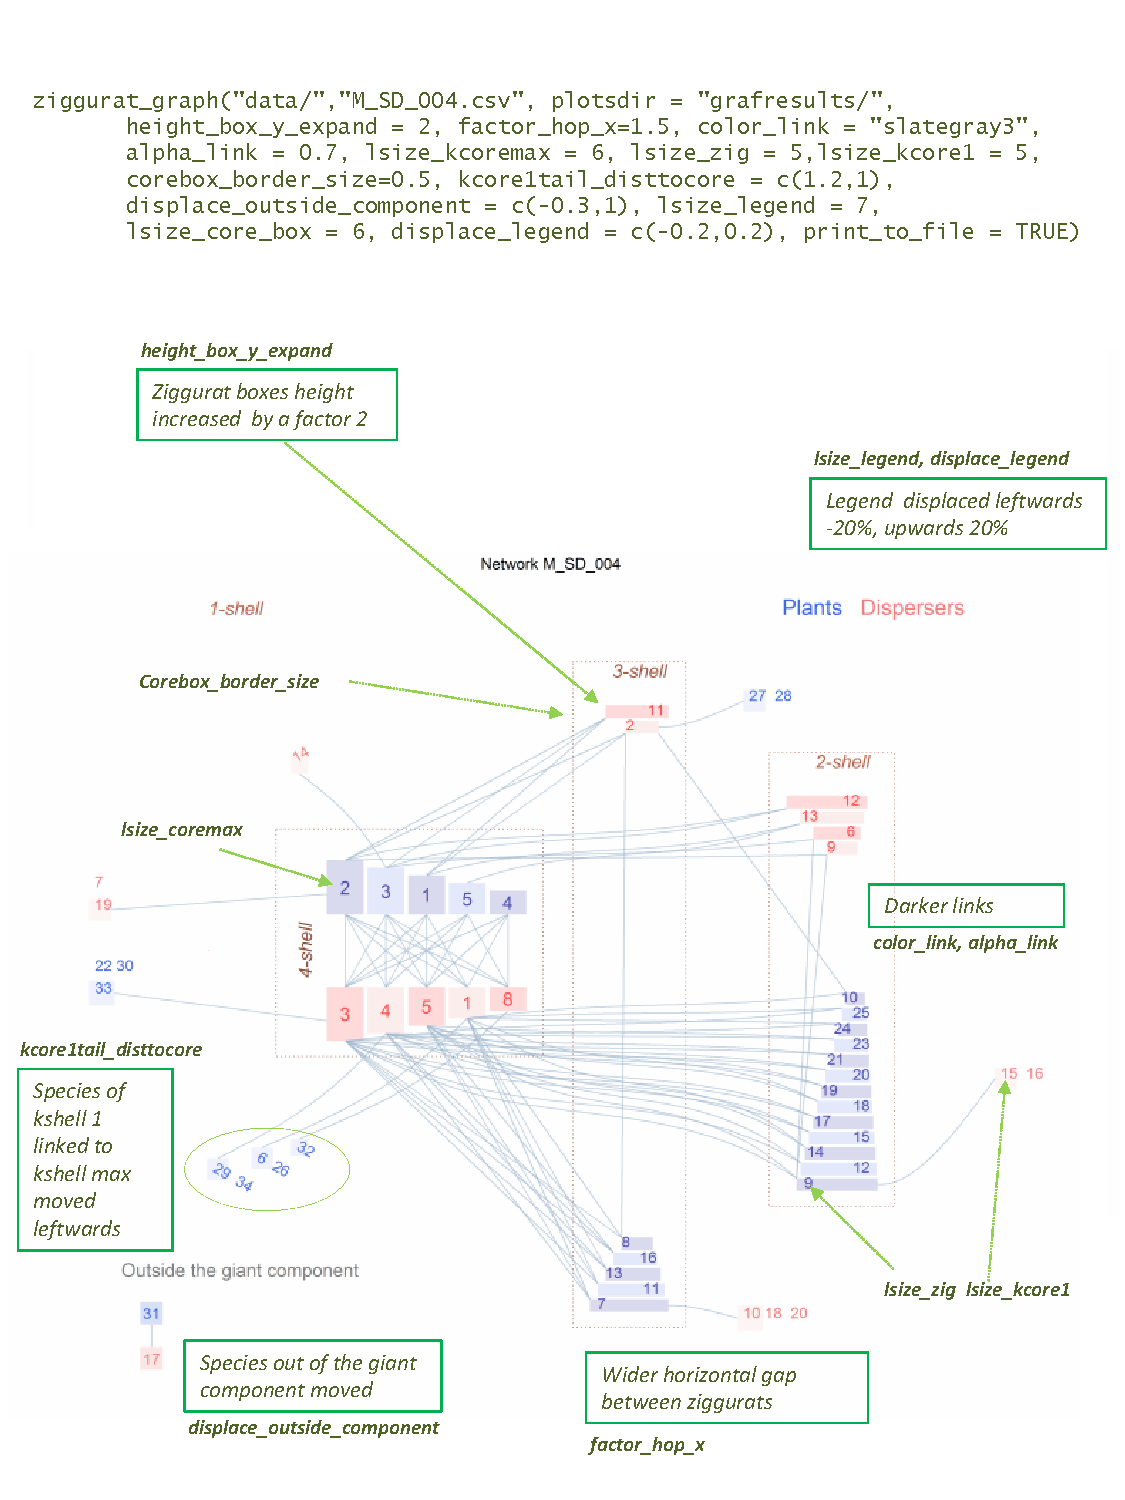
\includegraphics[scale=0.75]{M_SD_004_ziggurat_improved.pdf}
%\caption {Ziggurat graph of an avian frugivore community in Puerto Rico with 54 species and 95 links\cite{carlo2003avian}.}
\label{fig:ziggurat}
\end{figure}

\clearpage
Plot configuration may become quite complicated when network size grows, but we will show now the usefulness of another set
of input parameters with a medium size example. Default function call provides a quite readable ziggurat plot of pollinator
network number $12$.

\fontsize{3.5mm}{3.5mm}\selectfont
\begin{verbatim}
ziggurat_graph("data/","M_PL_012.csv",  plotsdir = "grafresults/", 
                print_to_file = TRUE)
\end{verbatim}
\normalsize

\begin{figure}[hp!]
\centering
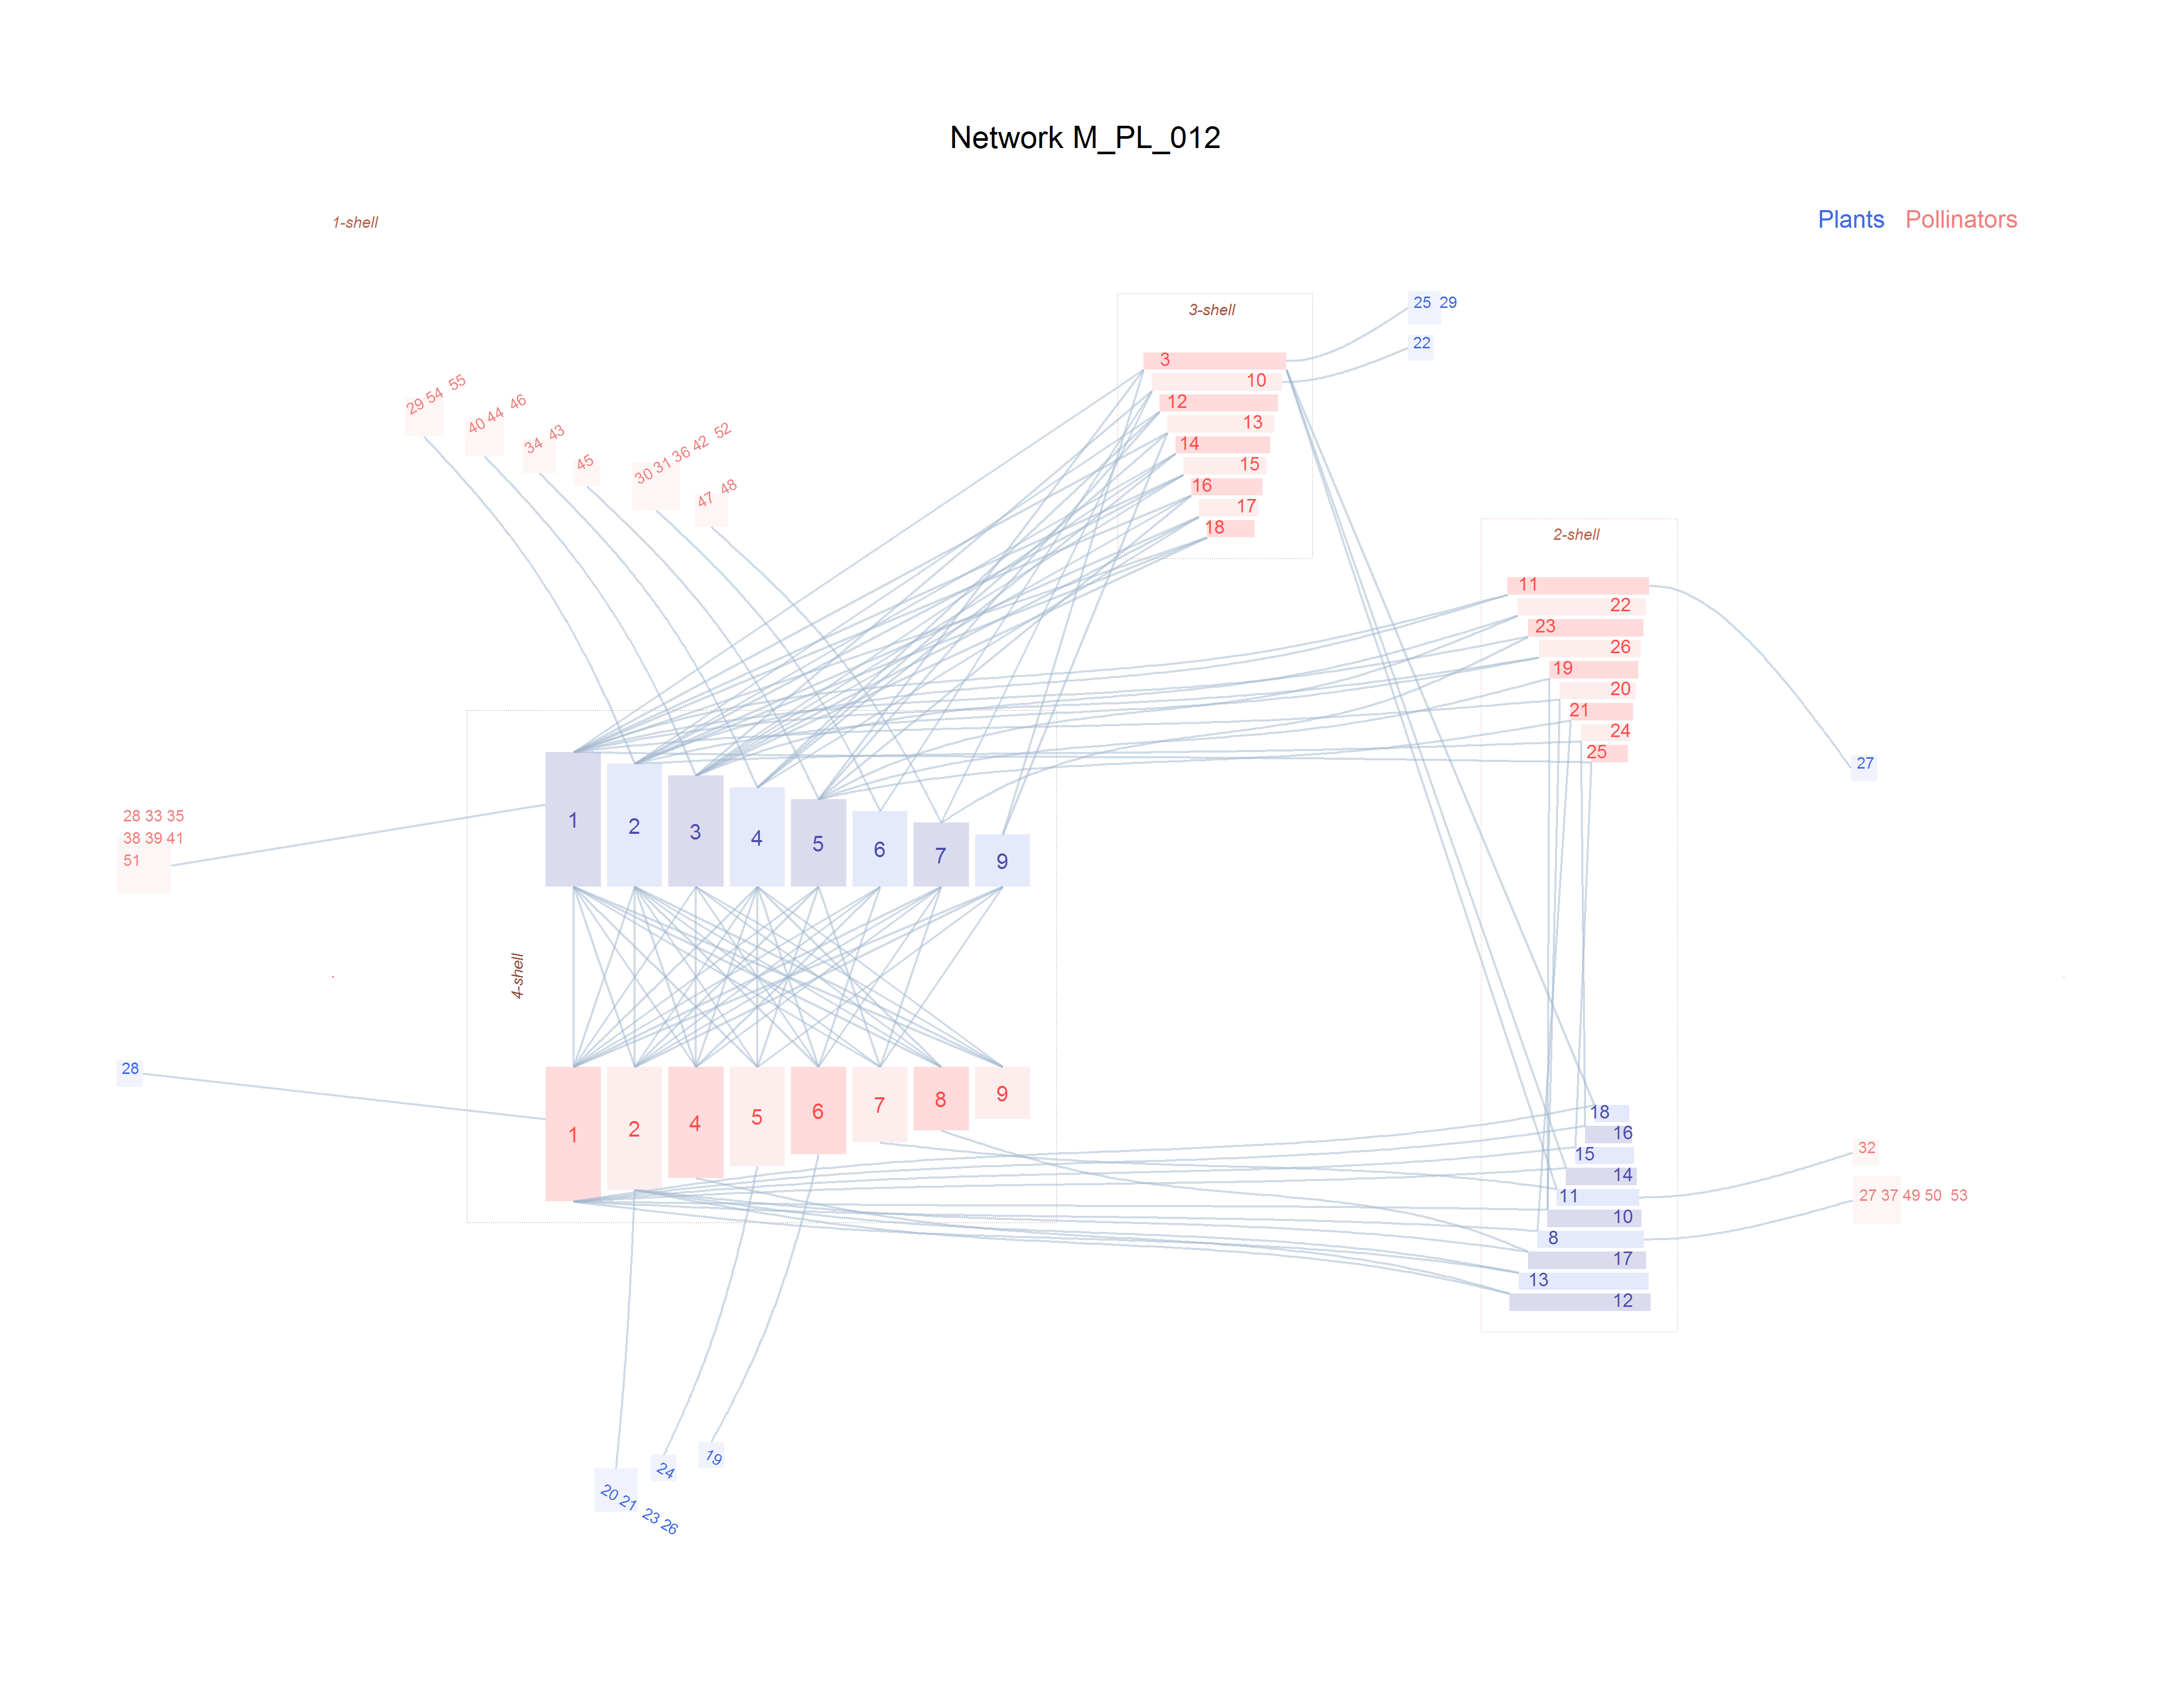
\includegraphics[scale=0.4]{M_PL_012_ziggurat.png}
\caption {Ziggurat graph of a plant - pollinator network in Garajonay, La Palma (Spain). Olesen, unpublished.}
\label{fig:ziggurat_012}
\end{figure}

This plot is nearly ready for publishing, some minor improvements would be nice, for instance increasing label sizes. However
we are going to modify several input values to show how the picture changes.

\clearpage
\begin{figure}[hbt!]
\centering
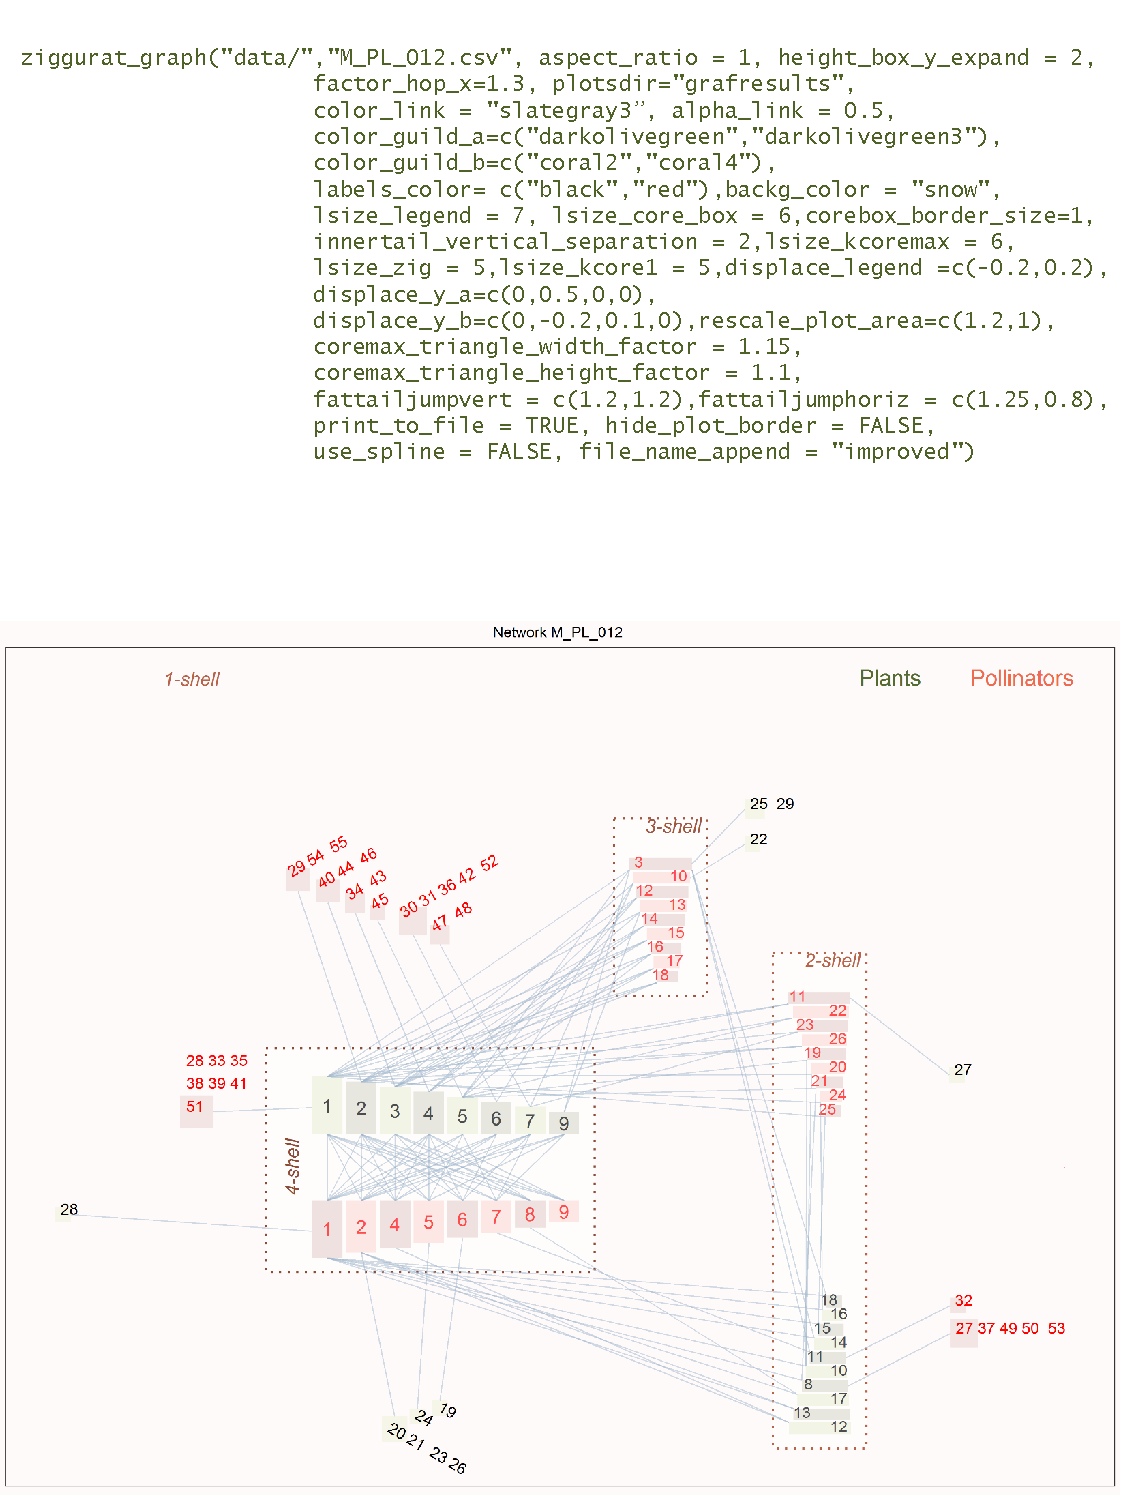
\includegraphics[scale=0.75]{M_PL_012_ziggurat_improved.pdf}
%\caption {Ziggurat graph of an avian frugivore community in Puerto Rico with 54 species and 95 links\cite{carlo2003avian}.}
\label{fig:ziggurat_012_improved}
\end{figure}

\clearpage
We will not repeat the meaning of those that we have explained in the previous example. The meaning of some of the new ones are quite
evident. We have changed the filling colors of ziggurats, providing the pairs \texttt{color\_guild\_a} and \texttt{color\_guild\_b},
and also the species label colors. A dime background is added as well. This trick shows the plotting area, that was horizontally increased
a $20\%$ with \texttt{rescale\_plot\_area=c(1.2,1)}. This change only affects the plotting area, not the the figure. The aspect ratio may
be modified to \textit{flatten} the plot is is lesser than $1$ or to \textit{stretch} it if bigger. The default value is $1$, it is not mandatory
to include, but we have added it to explain its meaning.

If you do not use splines, as in this example, links appear as straight lines. If you use splines you could also tell the function how many points they should have.

\textit{Fat tails} are the two sets of \textit{1-shell} species eventually linked to highest degree generalists, those that are located
leftmost in the max \textit{k-shell}. We may modify the vertical and horizontal distances to those species with \texttt{fattailjumpvert}
and \texttt{fattailjumphoriz}. Compare the relative position of plant species $28$ in this plot with the deafult one.

We saw how \texttt{height\_box\_y\_expand} controls the height of outer ziggurat boxes. Height and width of rectangles of the max \textit{k-shell} are modified with \texttt{coremax\_triangle\_height\_factor} and \texttt{coremax\_triangle\_width\_factor}. 

The overall horizontal distance of \textit{1-shell} species linked to max \textit{k-shell} (except fat tails) is increased or decreased with
\texttt{horiz\_kcoremax\_tails\_expand}.

Vertical separation of inner ziggurats is changed with vectors \texttt{displace\_y\_a} and \texttt{displace\_y\_b}. In this example, ziggurat
of \textit{2-shell} plants is moved upwards by a $50\%$,  \textit{2-shell} pollinators downwards $20\%$ and  \textit{3-shell} pollinators upwards $10\%$.

Finally, vertical separation of tails connected to inner ziggurats is increased with \texttt{innertail\_vertical\_separation}. See plant
species $22$ and $25$.

Next example shows how to manage \textit{weird tails} and \textit{outsiders}. Weird tails are chains of species of \textit{1-shell}. They
are rather unstable so they do not appear frequently. Outsiders are the species not connected to the giant component. Pollinator network $031$
has species of both kinds.

\clearpage
\begin{figure}[hp!]
\centering
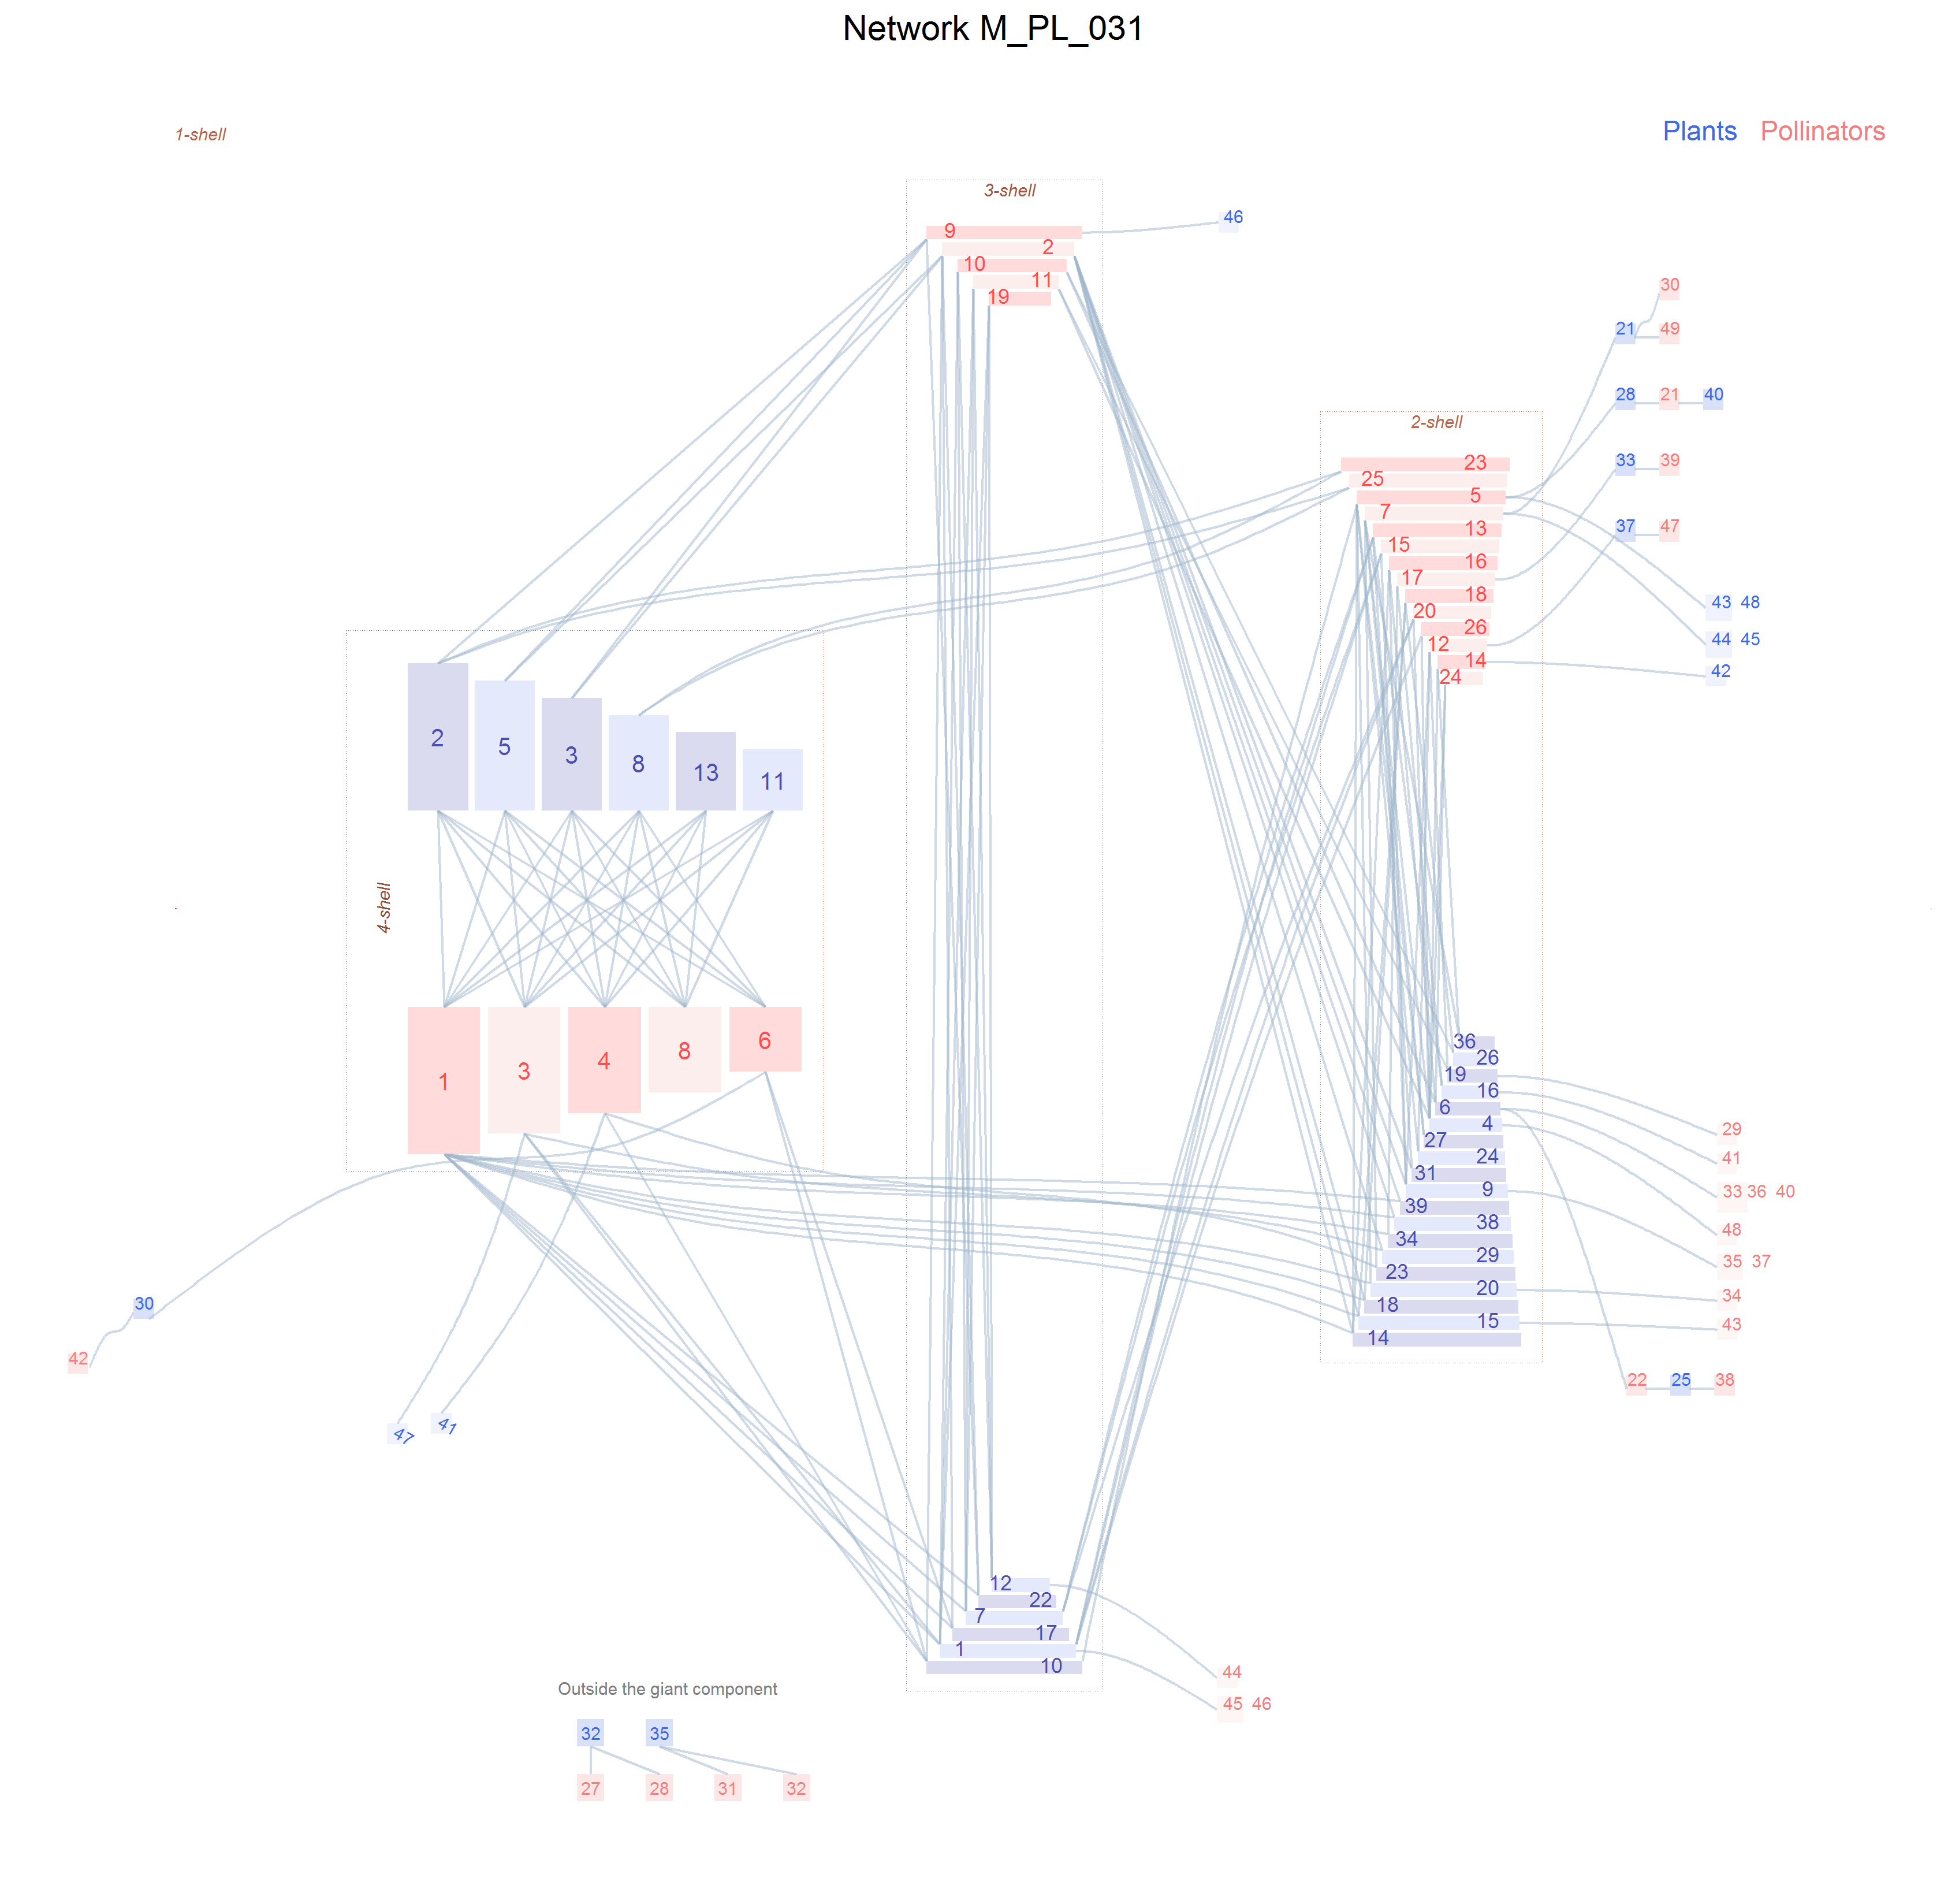
\includegraphics[scale=0.45]{M_PL_031_ziggurat.png}
\caption {Default ziggurat graph of a plant - pollinator network in Alta Guyana (Venezuela) \cite{ramirez1989biologia}.}
\label{fig:ziggurat_031}
\end{figure}

Outsiders appear under the main plot. This network has a rich set of weird chains, linked both to ziggurats of \textit{2-shell} and to the
max \textit{shell}. If plant species $28$ becomes extinct, it will also drag pollinator $21$ and plant $40$. This is an uncommon chain of
specialists linked among them and very exposed to external perturbations.

The \texttt{ziggurat\_grap} function offers input fields to manage the appearance and position of these species.

\clearpage
\begin{figure}[hp!]
\centering
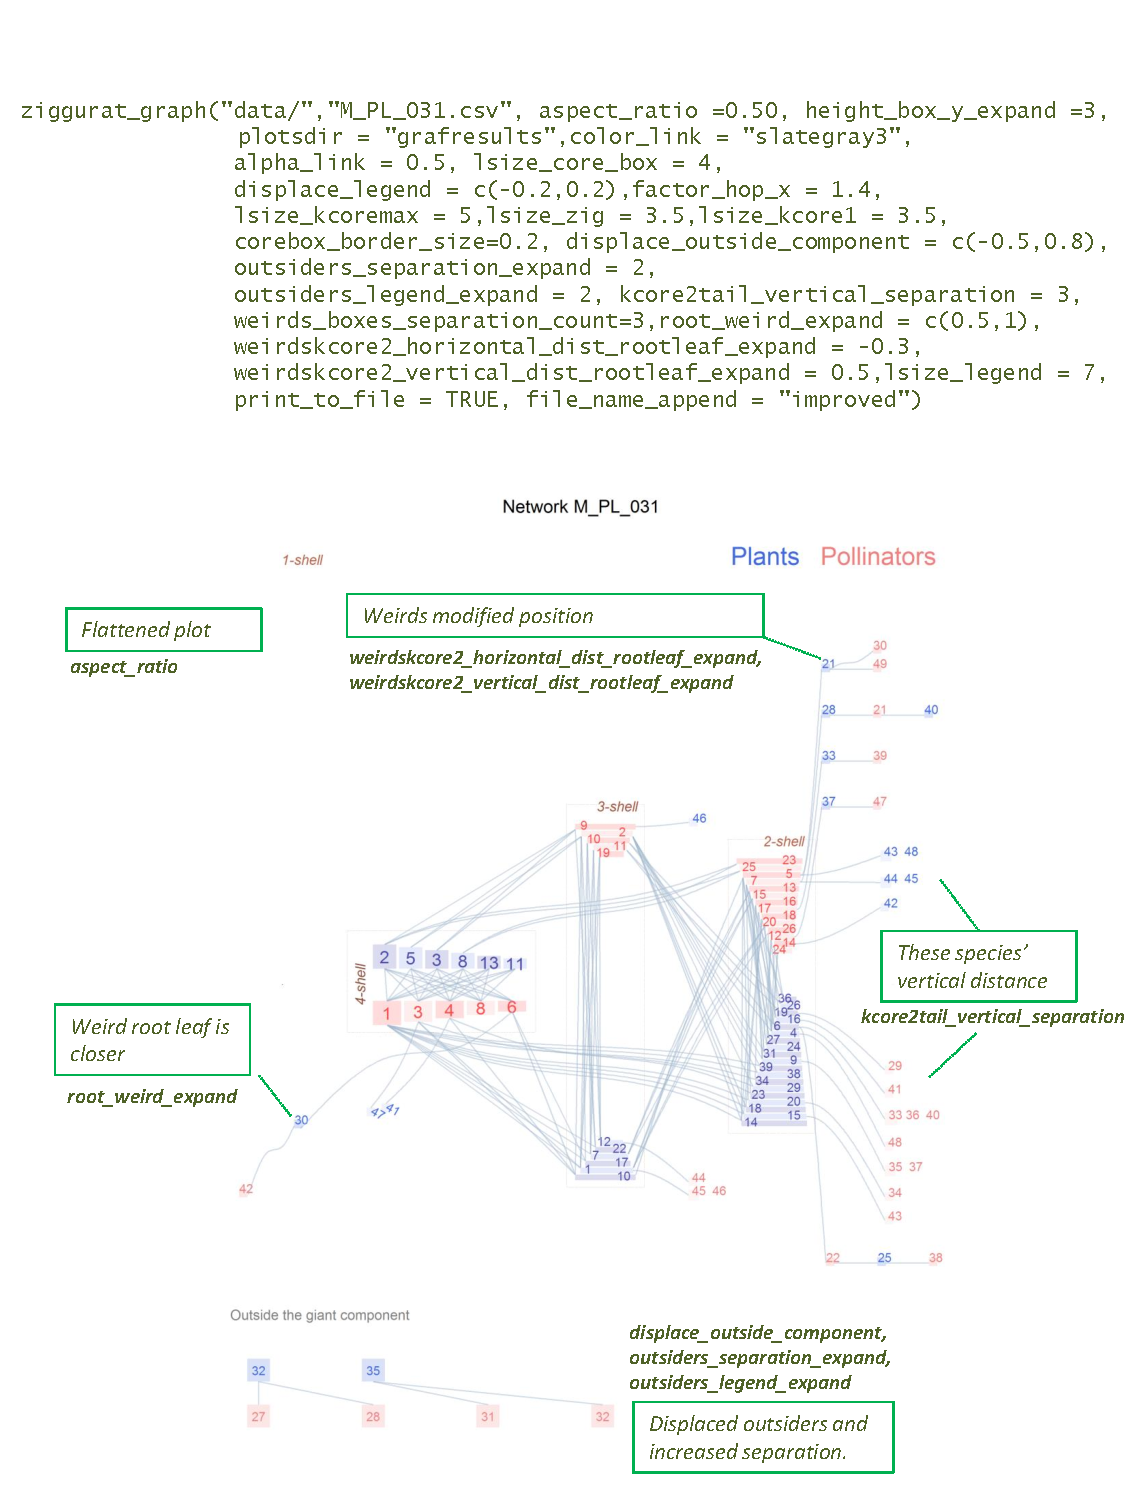
\includegraphics[scale=0.8]{M_PL_031_ziggurat_improved.pdf}
%\caption {Default ziggurat graph of a plant - pollinator network in Alta Guyana (Venezuela) \cite{ramirez1989biologia}.}
\label{fig:ziggurat_031}
\end{figure}


\clearpage

It is possible to display the names of the species inside the ziggurat rectangles. Be careful, because they may make
very difficult to understand the structure, we do not encourage using this feature unless the network is tiny. Species
names of \textit{1-shell} cannot be displayed

\begin{figure}[hp!]
\centering
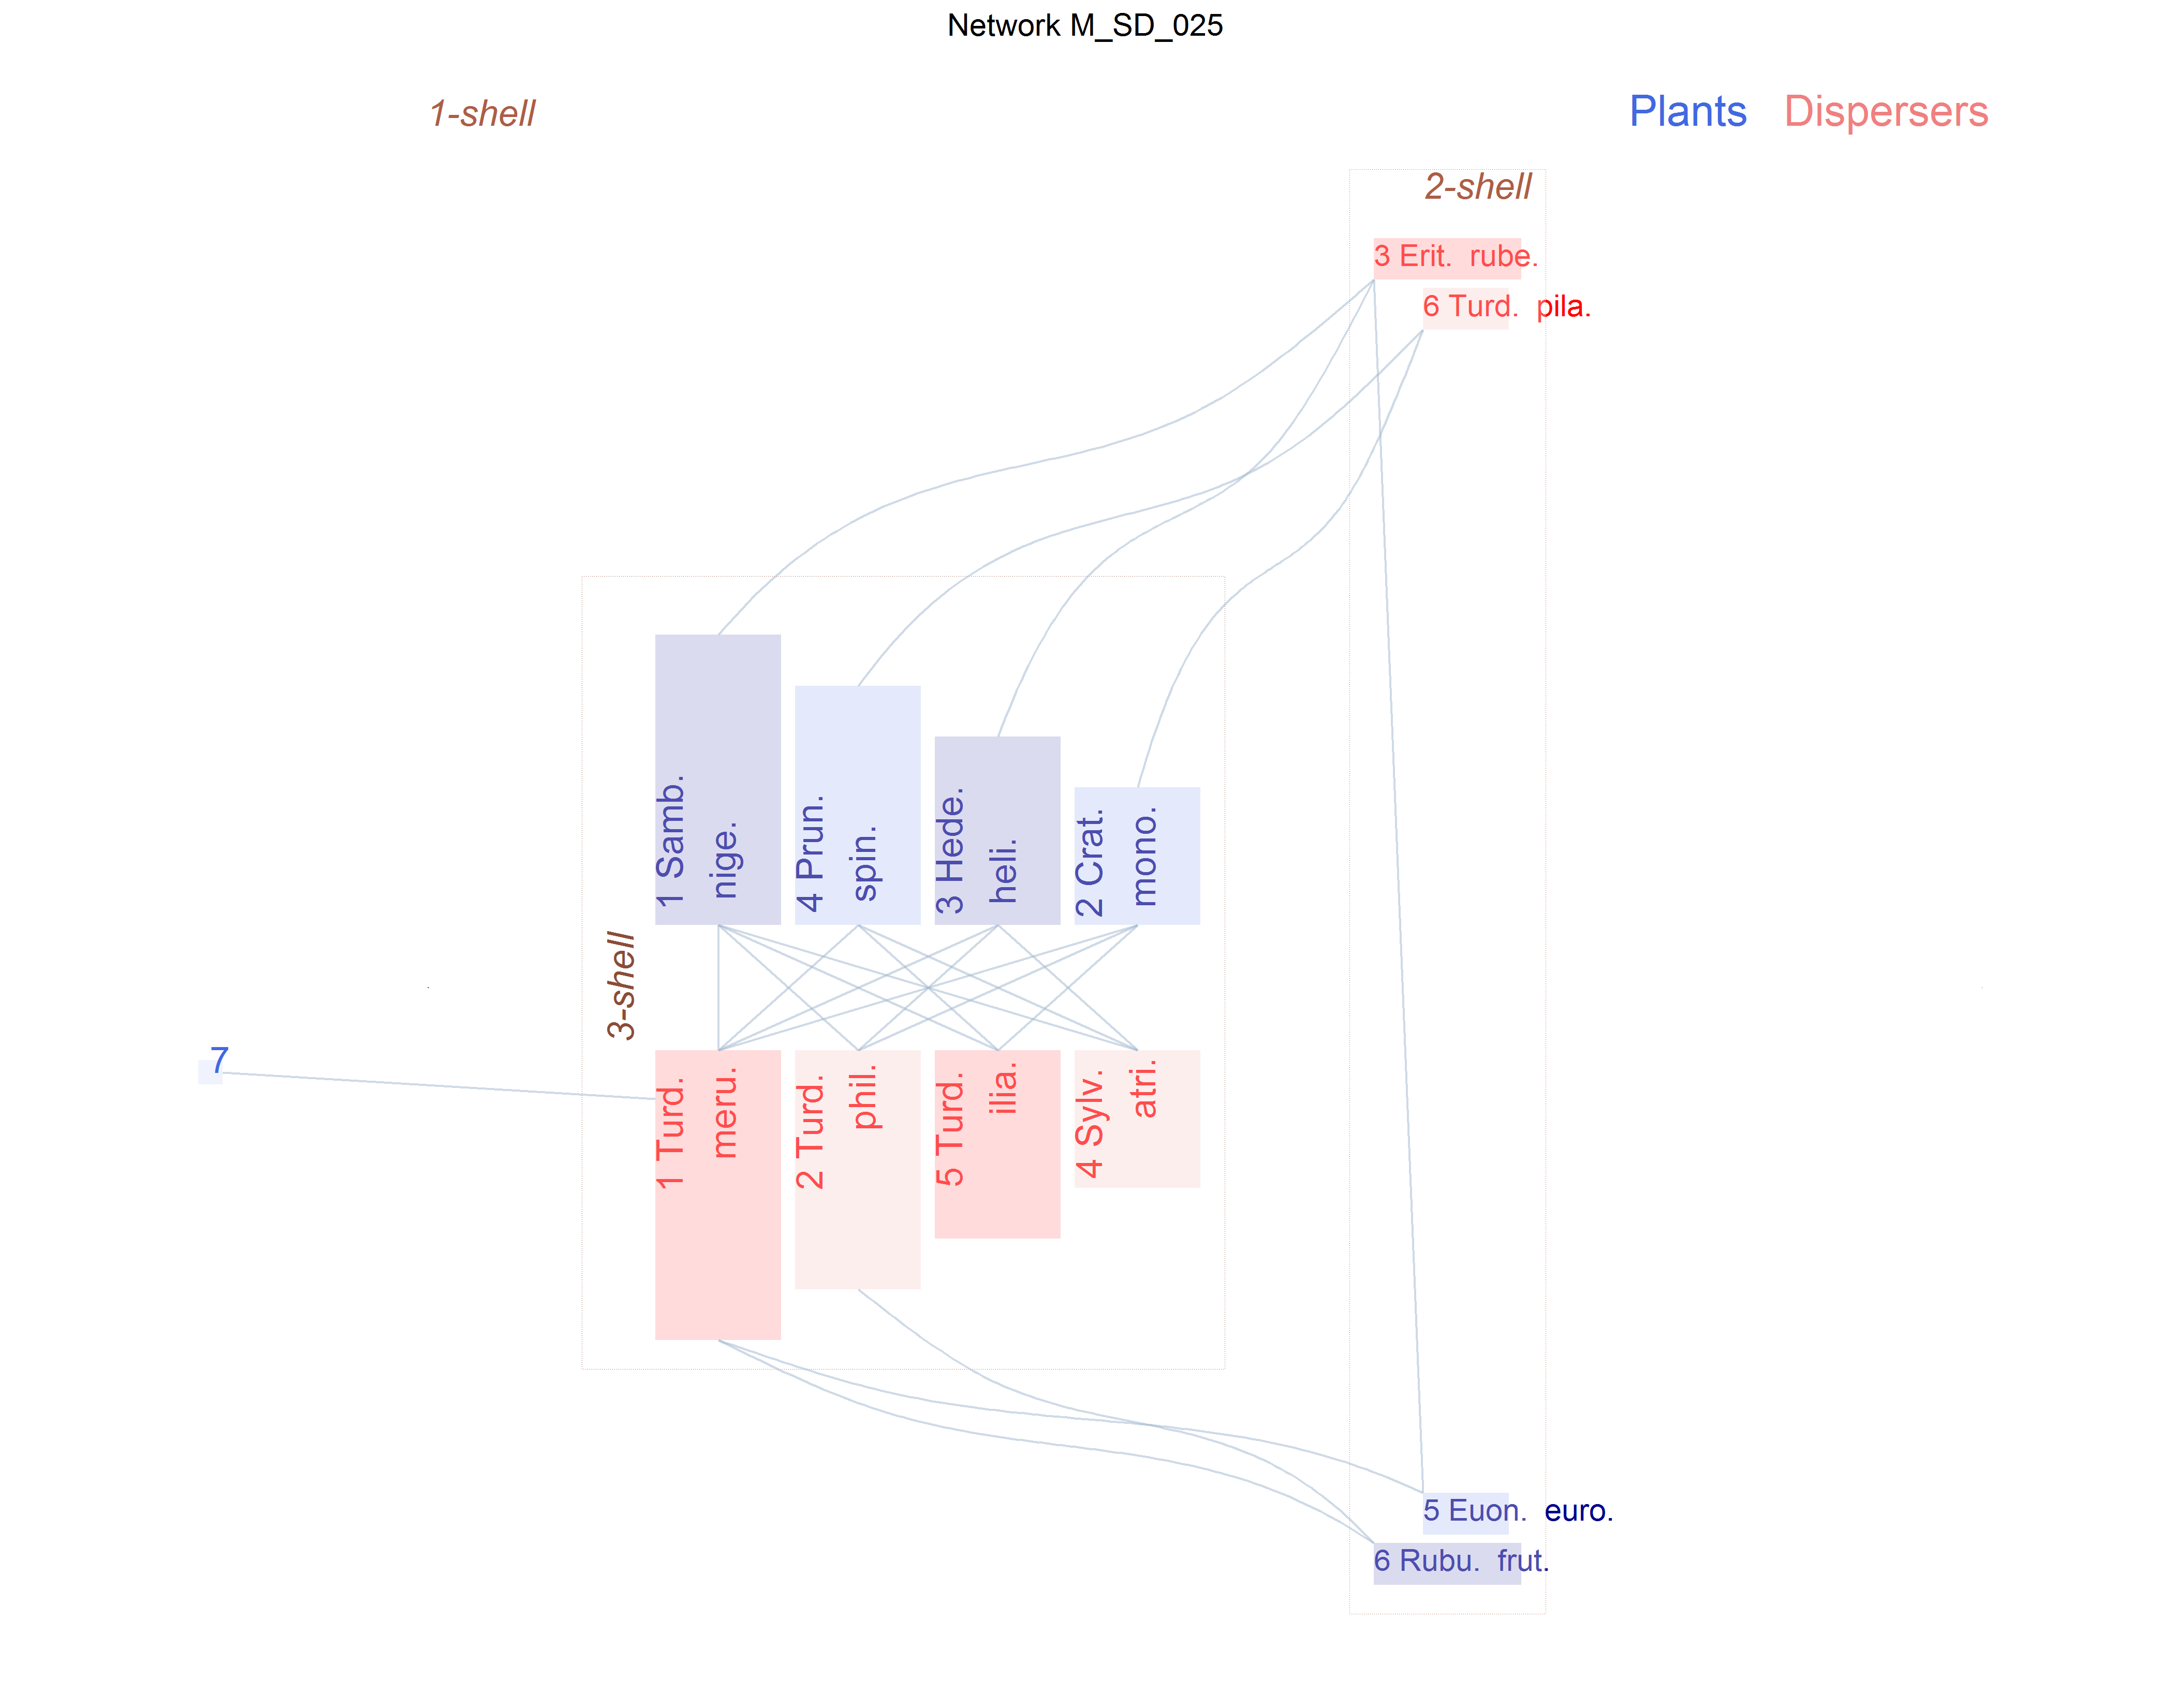
\includegraphics[scale=0.4]{M_SD_025_ziggurat.png}
%\caption {Default ziggurat graph of a plant - pollinator network in Alta Guyana (Venezuela) \cite{ramirez1989biologia}.}
\label{fig:ziggurat_025}
\end{figure}

\fontsize{3.5mm}{3.5mm}\selectfont
\begin{verbatim}
ziggurat_graph("./data/","M_SD_025.csv",plotsdir="grafresults/",
               shorten_species_name = 4, displace_legend = c(-0.2,0.2),
               height_box_y_expand = 2, coremax_triangle_width_factor = 1.25,
               coremax_triangle_height_factor = 2.25,lsize_core_box = 6,
               lsize_kcoremax = 6, lsize_legend= 7,lsize_kcore1 = 6, 
               lsize_zig = 5, kcore_species_name_display = c(2,3), 
               kcore_species_name_break = c(3), print_to_file = TRUE)

\end{verbatim}
\normalsize

\clearpage

\noindent The function returns its own environment called \texttt{zgg} where configuration paramenters and results
are stored. If you are developing an application, you can retrieve:

\begin{itemize}

\item \texttt{zgg\$plot}:  the ziggurat plot.

\item \texttt{zgg\$svg}: the ziggurat plot as an SVG object.

\item \texttt{zgg\$results\_analysis}: the internal \texttt{analyze\_network} call results.

\end{itemize}
 

\noindent Finally, this is the meaning of all the input parameters:
\small
\begin{itemize}

\item \texttt{datadir}:  name of the file of the interaction matrix.

\item \texttt{filename}: file with the interaction matrix.

\item \texttt{print\_to\_file}: if set to FALSE the plot is displayed in the R session window.

\item \texttt{plotsdir}:  the directory where the plot is stored.

\item \texttt{flip\_results}: displays the graph in portrait configuration.

\item \texttt{aspect\_ratio}: ziggurat plot default aspect ratio.

\item \texttt{alpha\_level}: transparency for ziggurats' filling.

\item \texttt{color\_guild\_a}: default filling for nodes of guild\_a.

\item \texttt{color\_guild\_b}: default filling for nodes of guild\_b.

\item \texttt{color\_link default}: link color.

\item \texttt{alpha\_link}: link transparency.

\item \texttt{size\_link}: width of the links.
\item \texttt{displace\_y\_b}: relative vertical displacement of guild\_b inner ziggurats.

\item \texttt{displace\_y\_a}: relative vertical displacement of guild\_a inner ziggurats.

\item \texttt{labels\_size}: default nodes labels size.

\item \texttt{lsize\_kcoremax}: nodes in kshell max label size.

\item \texttt{lsize\_zig nodes}: in inner ziggurats label size.

\item \texttt{lsize\_kcore1}: labels of nodes in kshell 1.

\item \texttt{lsize\_legend}: legend label size.

\item \texttt{lsize\_kcorebox}: default kshell boxes label size.

\item \texttt{labels\_color}: default label colors.

\item \texttt{height\_box\_y\_expand}: expand inner ziggurat rectangles default height by this factor.

\item \texttt{kcore2tail\_vertical\_separation}: expand vertical of kshell 1 species linked to kshell 2 by this factor.

\item \texttt{kcore1tail\_disttocore}: expand vertical separation of kshell 1 species from kshell max (guild\_a, guild,b).

\item \texttt{innertail\_vertical\_separation}: expand vertical separation of kshell species connected to 2 < kshell < kshell max.

\item \texttt{horiz\_kcoremax\_tails\_expand}: expand horizontal separation of weird tails connected to kshell max.

\item \texttt{factor\_hop\_x expand inner}: ziggurats horizontal distance.

\item \texttt{displace\_legend modify}: legend position by these fractions.

\item \texttt{fattailjumphoriz}: displace kshell 1 species linked to leftmost kshell max species.

\item \texttt{fattailjumpvert}: idem for vertical position.

\item \texttt{coremax\_triangle\_width\_factor}: expand khsell max rectangles width by this factor.

\item \texttt{coremax\_triangle\_height\_factor}: expand khsell max rectangles height by this factor.

\item \texttt{paint\_outsiders}: paint species not connected to giant component.

\item \texttt{displace\_outside\_component}: displace outsider species (horizontal, vertical).

\item \texttt{outsiders\_separation\_expand}: multiply by this factor outsiders' separation.

\item \texttt{outsiders\_legend\_expand}: displace outsiders legend.

\item \texttt{weirdskcore2\_horizontal\_dist\_rootleaf\_expand}: expand horizontal distance of weird tail root node connected to kshell 2.

\item \texttt{weirdskcore2\_vertical\_dist\_rootleaf\_expand}: expand vertical distance of weird tails connected to kshell 2.

\item \texttt{weirds\_boxes\_separation\_count}: weird species boxes separation count.

\item \texttt{root\_weird\_expand}: expand root weird distances of tails connected to kshell != 2.

\item \texttt{hide\_plot\_border}: hide border around the plot.

\item \texttt{rescale\_plot\_area}: full plot area rescaling (horizontal, vertical).

\item \texttt{kcore1weirds\_leafs\_vertical\_separation}: expand vertical separation of weird tails connected to kshell 1 species.

\item \texttt{corebox\_border\_size}: width of kshell boxes.

\item \texttt{kcore\_species\_name\_display}: display species names of shells listed in this vector.

\item \texttt{kcore\_species\_name\_break}: allow new lines in species names of shells listed in this vector.

\item \texttt{shorten\_species\_names}: number of characters of species name to display.

\item \texttt{label\_strguilda}: string labels of guild a.

\item \texttt{label\_strguildb}: string labels of guild b.

\item \texttt{landscape\_plot}: paper landscape configuration.

\item \texttt{backg\_color}: plot background color.

\item \texttt{show\_title}: show plot title.

\item \texttt{use\_spline}: use splines to draw links.

\item \texttt{spline\_points}: number of points for each spline.

\item \texttt{file\_name\_append}: a label that the user may append to the plot file name for convenience.

\item \texttt{svg\_scale\_factor}: only for interactive apps, do not modify.

\item \texttt{progress}: only for interactive apps, do not modifiy.
\end{itemize}


\normalsize

\clearpage
\printbibliography[heading=bibintoc]

\end{document}
